\documentclass{article}
\usepackage{amsmath}
\usepackage{graphicx}
\usepackage{listings}
\usepackage{nopageno}

\pagestyle{empty}
\begin{document}

\section*{PROBLEM STATEMENT}
To implement 2D translation transformation using OpenGL in C and to draw and translate a polygon against a defined coordinate system. The program will also draw the coordinate axes for better visualization.

\section*{THEORY}
2D translation is a geometric transformation that moves an object from one location to another in a 2D plane. The translation is defined by a translation vector \((t_x, t_y)\), which specifies the distance to move the object along the x-axis and y-axis.

The translation transformation matrix is given by:
\[
T = \begin{bmatrix}
1 & 0 & t_x \\
0 & 1 & t_y \\
0 & 0 & 1
\end{bmatrix}
\]

When a point \((x, y)\) is translated, the new coordinates \((x', y')\) are computed as:
\[
x' = x + t_x
\]
\[
y' = y + t_y
\]

\section*{ALGORITHM}

\begin{enumerate}
    \item Initialize the coordinates of the polygon vertices.
    \item Draw the coordinate axes using the Bresenham line drawing algorithm.
    \item Draw the original polygon.
    \item Apply the translation transformation to each vertex of the polygon.
    \item Draw the translated polygon in a different color.
\end{enumerate}

\section*{FLOWCHART}
\begin{center}
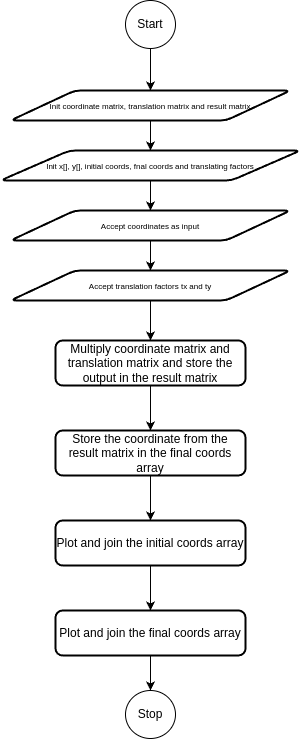
\includegraphics[width=0.7\textwidth]{flowchart.png}
\end{center}

\section*{SAMPLE I/O}
\textbf{Input:}
\begin{verbatim}
Polygon vertices: (10, 10), (200, 10), (200, 200), (10, 200)
Translation vector: tx = 40, ty = 50
\end{verbatim}

\textbf{Output:}
The original and translated polygons are displayed in a window with coordinate axes.

\section*{DISCUSSIONS}
\begin{itemize}
    \item \textbf{Advantages}: Translation is a simple and efficient transformation that is easy to implement. It is useful in various applications such as moving objects in graphics and animations.
    \item \textbf{Disadvantages}: Translation does not change the shape or size of the object, only its position.
    \item \textbf{Applications}: Translation is widely used in graphics, animation, CAD software, and game development for moving objects and models.
\end{itemize}

\section*{CONCLUSION}
The 2D translation transformation is fundamental in computer graphics for moving objects. Implementing this transformation using OpenGL provides a visual understanding of how translation affects the position of a polygon. Drawing coordinate axes helps in better visualization of the transformation effects.


\end{document}
